\section*{Question 1.9}
From this question onwards we switched to coding in Ansi C. 

Our general purpose statml methods are gathered subfolder \textit{statml} and the more particular functions for the assignments at hand are to be found in the \textit{common case.h} and \textit{common case.c} files respectively.
PNM image format handling is provided by a custom library provided in the files \textit{pnm.h} and  \textit{pnm.c}.

The GSL library is required to compile all of the above and the gnuplot program is required to generate to iso-probability curves for questions 1.10 and 1.11.

Given that the above requirements are met, the three programs for subassignments 1.9, 1.10 and 1.11 should compile by writing \textit{make run\_all} in a shell.

Have a look at the source code in mycase9.c for the sequence of operations performed to generate the sample mean of:
\cninesmean{}
and the covariance of:
\cninescov{}
from the training set.

These are then used as input for the Probability Density Function, as given in the assignment, which is run on every pixel to generate a density map. The density map is normalized to $[0\cdots255]$ and output as the following grayscale image:
\begin{center}
\includegraphics[width=0.5\textwidth]{dimg/case9probmap1.pdf}
\end{center}
It can be seen from the image above that not all pixels of the pitcher are distinctly capture by this approach. The picture appears to have been taken with a flash, providing a uniform hue distribution across most of the pitcher. The exception are where the surface points most away from the camera, which have a darker hue of red.

\section*{Question 1.10}
The weighted average position is calculated from the probability density map with the formula given in the assignment with the result:
\ctenwmean{}
The weighted average position is then used to calculate the spatial covariance:
\ctenwcov{}
Our program generates two datafiles are then generated for plotting by gnuplot. One  contains a presentation of the background image and the other a probability density map generated from the weighted average position and spatial covariance given above. The file \textit{plot.gnu} is a gnuplot script that uses the two files mentioned above to generate the following image:

\includegraphics[width=0.8\textwidth]{tex_out/case10.pdf}
The iso-probability curves in the resulting plot seem to capture the distribution of "pitcher coloured" pixels in the given image. The weighted average position has been plotted as a green square and seems to be aligned correctly at the center of the iso-probability curves.

\section*{Question 1.11}
When applying our sample mean and covariance from kande1 on kande2, we get the following weighted average position:
\celevenwmean{}
and the following spatial covariance:
\celevenwcov{}
Plotting these as iso-probability curves on top of kande2 gives the following image:

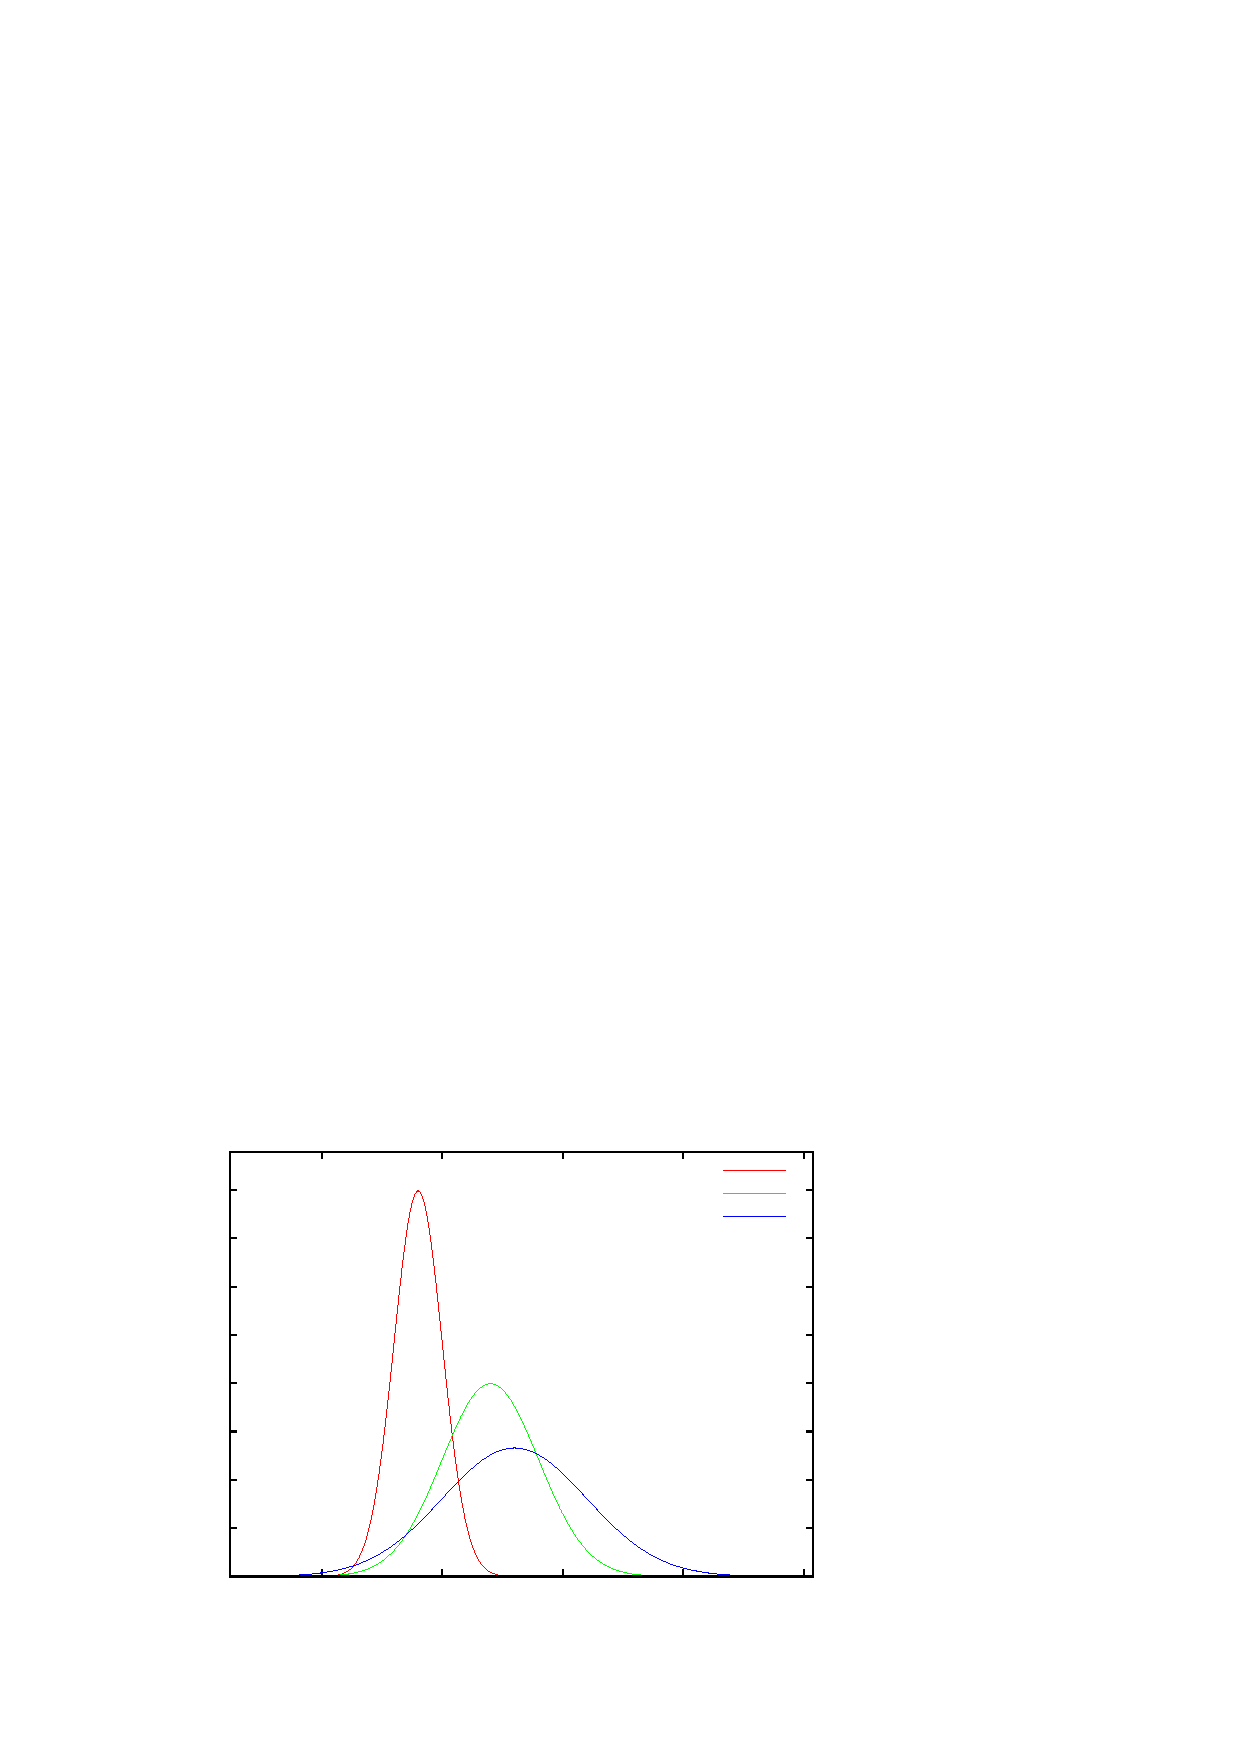
\includegraphics[width=0.8\textwidth]{tex_out/case11.pdf}

It is evident that the pitcher surface of kande2 is a lot less uniform than kande1, and it seems our model has recognized the collection of pixels with a similar colour distribution to that of the training set in kande1.

It seems that this approach is not able to reliably detect the outline of the red pitcher in the kande2 image with training data from the kande1 image.